\chapter{ENTANGLEMENT ENTROPY}
\label{chap:coupling}

% By labeling the chapter, I can refer to it later using the
% label. (\ref{chap:intro}, \pageref{chap:intro}) Latex will take care
% of the numbering.

In this chapter I will explain in detail the method we will use to generate 
evidence our nuclear wavefunctions can be 
significantly truncated. We will use the entanglement entropy of protons and
neutrons (the entropy of entanglement between protons and neutrons) to do this.

The entanglement entropy is a way to quantify the distribution of wavefunction
coefficients. Entanglement entropy pertains to bipartite systems, Hilbert spaces
with more than one species of wavefunction that can be represented as an outer product
of two or more subsystems. For us this means that our total Hilbert $\mathcal{H}^{\pi\nu}$ is the 
outer product of the subspace of many-proton states $\mathcal{H}_\pi$ with the
subspace of many-neutron states $\mathcal{H}_\nu$:
\begin{equation}
    \mathcal{H}^{\pi\nu} = \mathcal{H}_\pi\otimes\mathcal{H}_\nu.
\end{equation}
This is congruent with the fact that our basis states are written as outer products 
of proton and neutron Slater determinants. 
It will be shown that a wavefunction with zero proton-neutron entanglement entropy
can be written with a single term in an expansion such as (\ref{refEE2}). To 
do this I will first explain how the proton-neutron entanglement entropy comes
naturally out of a singular value decomposition of the coefficients 
of a wavefunction in a basis of coupled proton and neutron wavefunctions.

A singular value decomposition is a factorization of any matrix $A$ into the following
form:
\begin{equation}
    A = UDV^\dagger,
\end{equation}
where $U$ and $V$ are unitary matrices and $D$ is a diagonal matrix. 
The diagonal elements of $D$ are the SVD eigenvalues. See Appendix
\ref{appendix: svd} for more information about singular value decompositions. 
The matrices don't have to be square. Notice that if we compute $AA^\dagger$ we find:
\begin{equation}\begin{split}\label{svd1}
    AA^\dagger &=   UDV^\dagger   (UDV^\dagger)^\dagger\\
               &=   UDV^\dagger    VD^\dagger U^\dagger \\
               &=  UD D^\dagger U^\dagger,
\end{split}\end{equation}
where now $D^\dagger D =D^2$ is diagonal, square, and positive definite. 
The SVD eigenvalues $\gamma_i$ can thus be obtained from the diagonal elements 
$\gamma_i^2$ of $D^2$ by diagonalizing $AA^\dagger$ . Since equation (\ref{svd1})
represents a unitary transformation of a matrix, the SVD eigenvalues
are invariant. This means that the SVD eigenvalues of the coefficients in the 
expansion (\ref{eqn: decomptrunc}) can found by diagonalizing the matrix  
\begin{equation}\label{svd2}
    (AA^\dagger)_{a'a}=\sum_b\Psi_{a'b}\Psi^*_{ba},
\end{equation} 
from the coefficients in equation (\ref{eqn: decomp1}) which we can find
from solutions in a known basis.

Equation (\ref{svd2}) is simply the reduced density matrix of the eigenstate 
$\ket{\Psi}$ in the choice of basis given in (\ref{eqn: decomp1}). The 
\textit{density operator} of a pure state $\Psi$ is defined as 
\begin{equation}
    \rho = \ket{\Psi}\bra{\Psi}.
\end{equation}
Given the choice of basis shown in equation (\ref{eqn: decomp1}), we can compute 
the following density matrix:
\begin{equation}\label{rhoall}
    \rho_{a'b'ab} = {\Psi}_{a'b'}{\Psi}^*_{ba}.
\end{equation} 

If the Hilbert space is bipartite $\mathcal{H}^{\pi\nu} = \mathcal{H}^\pi \otimes \mathcal{H}^\nu$ 
then we can define the reduced density operator of a particular subspace $\mathcal{H}^\pi$ to be
the trace over the conjugate subspace $\mathcal{H}^\nu$:
\begin{equation}
    \rho^\pi = tr_\nu \rho^{\pi\nu},
\end{equation}
where $\rho^{\pi\nu}$ is a density operator in the space $\mathcal{H}^{\pi\nu}$
and the trace operator $tr_\nu$ contracts the indices belonging to the $\mathcal{H}^\nu$
Hilbert space.
The reduced density matrix $\rho^\pi$ in our choice of basis is computed from
(\ref{rhoall}):
\begin{equation}\begin{split}\label{matprod}
    \rho_{a'a}^{\pi} &= \sum_{b'b}\delta_{b'b} (\rho_{a'b'ab}) \\
        &=\sum_b {\Psi}_{a'b}{\Psi}^*_{ba}\\
        &=(AA^\dagger)_{a'a}.
\end{split}\end{equation}
In the SVD papers cited earlier, this density matrix was only used to 
compute the SVD eigenvalues. Here, we are going to take advantage of the information
of mixing that is contained within the density matrix: the entanglement entropy.

The \textit{von Neumann entropy} is defined in terms 
of the generalized density operator (quantum state $\rho$) by
\begin{equation}
    S(\rho) \equiv -tr(\rho\ \ln\rho).
\end{equation}
The \textit{entanglement entropy} of a state in a bipartite system 
$\mathcal{H}^{\pi\nu} = \mathcal{H}^\pi \otimes \mathcal{H}^\nu$ is the
von Neumann entropy of a reduced density matrix: 
\begin{equation}
    S(\rho^\pi) = -tr(\rho^\pi \ln \rho^\pi).
\end{equation}
In our case, the proton-neutron entanglement entropy
measures the number of quantum bits shared between the proton and neutron spaces.
It is also a measure of the distribution of the SVD eigenvalues. It can be shown 
that $S(\rho^\pi)=S(\rho^\nu)$, from the invariance of SVD eigenvalues.
We therefore simply refer to $S_{pn}\equiv S(\rho^\pi)=S(\rho^\nu)$ as the 
proton-neutron entanglement entropy.
We first diagonalize the density matrix $\rho_\pi$ and compute 
$S_{pn}$ using the eigenvalues $\{\gamma_i^2\}$ of $\rho_\pi$ so that
\begin{equation}
    S_{pn} = -\sum_i \gamma_i^2\ \ln(\gamma_i^2),
\end{equation}
where $\gamma_i$ are also the SVD eigenvalues of $\tilde{\Psi_{ab}}$ and
$\Psi_{i_pj_n}$.
The proton-neutron entanglement entropy for a given state $\ket{\Psi}$ 
is a measure of the entanglement of the two partitions of the Hilbert space. 
It indicates the degree to which an expansion 
\begin{equation}\label{diag}
    \ket{\Psi} = \sum_i \gamma_i \ket{\tilde{\pi}_i}\ket{\tilde{\nu}_i}
\end{equation}
can be truncated. 
If the entanglement entropy is zero, then (\ref{diag})
contains only one term. A maximal value of $S_{pn}$ would indicate that each 
term in the expansion is equally weighted; then we would have
\begin{equation}
    S_{max} = \ln(d_p).
\end{equation}


Let's consider a bipartite spin system $\mathcal{H}_{12}=\mathcal{H}_1\otimes
\mathcal{H}_2$ to illustrate this. We can represent any wavefunction in this
space as
\begin{equation}\label{matrepres}
    \ket{\Psi}=\sum_{ab}\Psi_{ab}\ket{a}\otimes\ket{b}\to \underline{\Psi} =
    \begin{bmatrix} \Psi_{\uparrow\uparrow}&\Psi_{\uparrow\downarrow}\\ 
    \Psi_{\downarrow\uparrow}&\Psi_{\downarrow\downarrow}\end{bmatrix},
\end{equation}
where the basis vectors $\ket{a}$ and $\ket{b}$ are either $\ket{\uparrow}$ or $\ket{\downarrow}$, and
where the elements of the matrix $\underline{\Psi}$ are the coefficients for the four possible bipartite
basis states.
Let's compute the entanglement entropy for two spin-1/2 particles which are not entangled: 
\begin{equation}\label{noentangle}
    \ket{\Psi}=\ket{\uparrow\downarrow}\to\underline{\Psi}=\begin{bmatrix}0&1\\0&0\end{bmatrix}.
\end{equation}
The reduced density matrix of this wavefunction can be computed as the matrix
product $\underline{\Psi}*\underline{\Psi}^\dagger$ (see equation (\ref{matprod})):
\begin{equation}
    \underline{\rho}_1 = \begin{bmatrix}0&1\\0&0\end{bmatrix} \begin{bmatrix}0&0\\1&0\end{bmatrix}=\begin{bmatrix}1&0\\0&0\end{bmatrix}.
\end{equation}
This density matrix is already diagonal, so we can compute its von Neummann entropy
as
\begin{equation}
    S_{12}=S(\rho_1) = -(1\ln(1)+0\ln(0)) = 0.
\end{equation}
Thus a non-entangled pair of spin-1/2 particles has zero entanglement entropy.

We can follow the same procedure for an entangled pair:
\begin{equation}\label{maxentangle}
    \ket{\Psi'}=\frac{1}{\sqrt{2}}(\ket{\uparrow\downarrow}-\ket{\downarrow\uparrow}),
\end{equation} 
which can be represented as a matrix using (\ref{matrepres}):
\begin{equation}
    \underline{\Psi'} = \frac{1}{\sqrt{2}}\begin{bmatrix}0&1\\-1&0\end{bmatrix}.
\end{equation}
The reduced density matrix is
\begin{equation}
    \underline{\rho'}=\underline{\Psi'}*\underline{\Psi'}^\dagger=\frac{1}{2}\begin{bmatrix}1&0\\0&1\end{bmatrix}.
\end{equation}
Thus this entangled pair has an entanglement entropy 
\begin{equation}
    S_{12}=S(\rho_1)=-(\frac{1}{2}\ln(\frac{1}{2})+\frac{1}{2}\ln(\frac{1}{2}))=\ln 2,
\end{equation}
which is the maximum entanglement entropy for a bipartite system with two-dimensional subspaces.

A lower proton-neutron entanglement entropy corresponds to a system in which we can obtain a more
accurate representation of our state $\ket{\Psi}$ with fewer states in (\ref{diag}).
The proton-neutron entanglement entropy has an advantage over the raw
distribution of SVD values because we can use it to compare multiple states with a single
number. In particular, if the proton-neutron entanglement entropy is smaller in 
nuclei where isospin is large, then we can expect such a truncation scheme to be more effective
for large isospin nuclei. This is good news for the calculation of large nuclei with a large 
excess of neutrons. Cesium 133 has $40\%$ more neutrons than protons, for example.
However, and this is critical, we do not yet have a criterion to find the optimal basis 
$\{\ket{\tilde{\pi}_i}\ket{\tilde{\nu}_i}\}$, we are only generating evidence
that one exists. 

We will compute the proton-neutron entanglement entropy and demonstrate that it is
significantly lower for $N>Z$ nuclei than for $N=Z$ nuclei, even for nuclei with the
same model space dimensions. First I will justify the use of low proton-neutron 
entanglement entropy as an indicator of the existence of a  basis which can yield
accurate truncated representations. 


\subsection{Particle-Hole Conjugates}
The proton-neutron entanglement entropy depends on the dimension of the 
model space. In order for the proton-neutron entanglement entropy to be useful in
comparing different nuclei, we need cases with equal or similar dimensionality. 
To do this, we choose to compare particle-hole conjugates. 

In the interacting shell model, 
we reduce the effective size of the Hilbert space by redefining the vacuum state 
to be some inert core of nucleons, above which is a system of interacting particles. 
Some interacting shell model codes can also carry out ``particle hole
conjugation''\cite{Brussard,Heyde}, where a system of particles can be
described instead by a system of holes. A hole is a gap in an otherwise filled shell.
The number of valence particles is restricted to some maximum value and a filled particle state
is mathematically equivalent to a hole. If a nucleus has fewer holes than particles
in a model space, it is preferable to model it as a system of interacting holes.
Two nuclei which are particle-hole conjugates in a model space have an equal
number of proton particles and/or proton holes, and an equal number of
neutron particles and/or neutron holes.

Consider the following example:
$^{18}$F in the \textit{sd}-shell ($0d_{3/2}$, $0d_{5/2}$ and $1s_{1/2}$) has 8 inert protons and 8 inert neutrons,
with one valence proton and one valence neutron, both of which are in the
$0d_{3/2}$ single particle orbit. The sd-shell model space has a maximum of 12 valence particles
of each type, since the space ($0d_{3/2}$, $0d_{5/2}$ and $1s_{1/2}$) has 12 unique
quantum numbers in $n$, $l$, $j$, $m$. Thus $^{18}$F has 12 possible states each for 
the proton and neutron. $^{38}$K, which has 11 valence protons and 11 valence neutrons, 
can be represented by two particle holes in the completely filled \textit{sd}-shell model space,
and thus also has 12 possible states. {Table \ref{table: sd.spo}} contains the complete set of
sd-shell model space quantum numbers.

Table \ref{tbl: log} is a collection of nuclei for which the proton-neutron 
entanglement entropy of the ground state were computed. Each row in the table
is a particle-hole conjugate triplet, meaning every nucleus is listed in the 
same row as its particle-hole conjugates. For example, $^{18}$F, $^{28}$F, and $^{38}$K
are particle-hole conjugates . The numbers to the right of each nuclide
are the number of valence protons ($Z_{val}$) and valence neutrons ($N_{val}$), 
respectively, in each nuclide's respective shell model space.

\begin{table}
    \caption{Table of Particle-Hole Conjugate Nuclei in the \textit{sd}-Shell Model Space}
    \label{tbl: log}
%\centering

\begin{tabular}
    {c | c c c c c c c}
    \hline 
    \hline
Inert Core & Nucleus & ($Z_{val}$, $N_{val}$) &  &  &  &  & $d_p=d_n$ \\
 
    \hline
$^{16}$O    &$^{18}$F   &(1,1)   & $^{28}$F   &(1,11) & $^{38}$K   &(11,11) & 12 \\
       &$^{20}$Ne  &(2,2)   & $^{28}$Ne  &(2,10) & $^{36}$Ar  &(10,10) & 66\\
       &$^{22}$Na  &(3,3)   & $^{28}$Na  &(3,9)  & $^{34}$Cl  & (9, 9) & 220\\
       &$^{24}$Mg  &(4,4)   & $^{28}$Mg  &(4,8)  & $^{32}$S   & (8, 8) & 495\\
       &$^{26}$Al  &(5,5)   & $^{28}$Al  &(5,7)  & $^{30}$P   & (7, 7) & 792\\
\hline                                                                          
$^{40}$Ca   &$^{42}$Sc  &(1,1)   & $^{60}$Sc  &(1,19) & $^{78}$Y   &(19,19) & 20 \\
       &$^{44}$Ti  &(2,2)   & $^{60}$Ti  &(2,18) & $^{76}$Sr  &(18,18) & 190 \\
       &$^{46}$V   &(3,3)   & $^{60}$V   &(3,17) & $^{74}$Rb  &(17,17) & 1140 \\
       &$^{48}$Cr  &(4,4)   & $^{60}$Cr  &(4,16) & $^{72}$Kr  &(16,16) & 4845 \\
\hline
$^{56}$Ni    &$^{58}$Cu  &(1,1)   & $^{78}$Cu  &(1,21) & $^{98}$In  &(21,21) & 22 \\
       &$^{60}$Zn  &(2,2)   & $^{78}$Zn  &(2,20) & $^{96}$Cd  &(20,20) & 231 \\
       &$^{62}$Ga  &(3,3)   & $^{78}$Ga  &(3,19) & $^{94}$Ag  &(19,19) & 1540 \\
       &$^{64}$Ge  &(4,4)   & $^{78}$Ge  &(4,18) & $^{92}$Pd  &(18,18) & 7315 \\
\hline
$^{100}$Sn  &$^{102}$Sb &(1,1)   & $^{132}$Sb &(1,31) & $^{162}$Ti &(31,31) & 32 \\
       &$^{104}$Te &(2,2)   & $^{132}$Te &(2,30) & $^{160}$Hg &(30,30) & 496 \\
       &$^{106}$I  &(3,3)   & $^{132}$I  &(3,29) & $^{158}$Au &(29,29) & 4960 \\
Figure \ref{pns: all} symbol: & Diamond && Circle && Square \\
    \hline
    \hline
\end{tabular}

\end{table} 

Figure \ref{pns: all} is a collection of proton-neutron entanglement entropies
for the nuclei listed in table \ref{tbl: log}. The vertical axis is the relative proton-
neutron entanglement entropy and each particle-hole conjugate triplet lies in a 
given column and is labeled according to its representative nucleus. Each row in 
table \ref{tbl: log} is plotted in its own column. For example, the data points
above $^{18}$F on the horizontal axis are $^{18}$F ($N=Z$), $^{28}$F ($N>Z$) and $^{38}$K ($N=Z$).
Each of the four frames in the Figure corresponds to a different shell-model space
listed in table \ref{tbl: log}.

Figure \ref{pns: all} demonstrates that nearly all particle-hole triplets in the 
four model spaces tested have the lowest proton-neutron entanglement entropy in
nuclei where $N>Z$. The exceptions are the $^{18}$F, $^{22}$Na, and $^{26}$Al triplets in the 
sd-shell model space and the $^{42}$Sc triplet in the \textit{pf}-shell model space.
All four of these exceptions are odd-odd nuclei. 

\begin{figure}
    \centering    
    \includegraphics[width=.75\textwidth,clip]{Figures/s_gs_full}
    \caption{Normalized proton-neutron entanglement entropy for nuclei listed in 
Table \ref{tbl: log}. The horizontal axis
labels particle-hole conjugate (PHC) triplets by the smallest nuclide in the 
leftmost column of Table \ref{tbl: log} and are sorted left to right by increasing 
\boldmath$S_{max}=\ln(\min[d_\pi,d_\nu])$.  In most cases within each PHC triplet, the nuclide with an unequal 
numbers of protons and neutrons has the lowest entanglement entropy. All exceptions include
nuclei with an odd-Z and odd-N (odd-odd) nuclide. (Circle: $N>Z$ nuclide, Square: heaviest PHC nuclide,
Diamond: lightest PHC nuclide.)}
    \label{pns: all}
\end{figure}

\subsection{Excited States and Thermalization}
In order for our approach to be viable, we will need the pattern exhibited in 
the previous sections to hold for not just the ground state, but for excited 
states as well. By plotting the proton-neutron entanglement entropy for
a number of the lowest energy levels, we see that $N>Z$ nuclei tend to have
the lowest proton-neutron entanglement entropies only for the first few 
lowest eigenstates. After this, the ordering becomes apparently random.
We came to the conclusion that we are observing a kind of thermalization. 
As the energy of the system increases,
the low entropy configurations expressed in $N>Z$ nuclei disappear. An example
is given in Figure \ref{smglvl}.

\begin{figure}[t]
    \centering
    \includegraphics[width=.75\textwidth,clip]{Figures/S_vs_level_mg}
    \caption{Proton-neutron entanglement entropy versus excitation level for $^{28}$Mg and 
its particle-hole conjugates in the \textit{sd}-shell. 
The entanglement entropy is lower in the $^{28}$Mg spectrum for the first ten 
excitation levels.}
    \label{smglvl}
\end{figure}

\subsection{Entropy and Isospin}
So far we have demonstrated on a case by case basis that $N>Z$ nuclei tend to have
lower proton-neutron entanglement entropy than their particle-hole conjugates. 
The next kind of plot that we examine are plots of proton-neutron entanglement 
entropy $S$ versus isospin, specifically the z-component of the isospin $T_z$. 
We will use the convention that for protons $T_z=-\frac{1}{2}$ and that for
neutrons $T_z=+\frac{1}{2}$. We can then compute the maximum value of $T_z$ for 
a given nucleus as $\frac{1}{2}(N-Z)$. As shown in Figures \ref{fig: tz1} as 
$T_z$ increases, the proton-neutron entanglement entropy tends to decrease. This
was shown in both the \textit{sd} shell and the \textit{pf} shell. We also extended the analysis 
to the sd-pf shell model space where we examined non physical nuclei with 
value of $T_z$ as high as $T_z=14$.

In Figure \ref{fig: tz1}, we see that odd-odd nuclei (nuclei with odd numbers of protons
and neutrons) have especially high proton-neutron entanglement. We hypothesize that
this is due to the pairing interaction, which describes a tendency for pairs
of nucleons to preferentially couple to $J=0$\cite{Brussard}. In odd-odd nuclei,
one proton and one neutron are left unpaired, and it is thus thought that the pairing
interaction leads to an increased interaction between these unpaired nucleons and
therefore a higher proton-neutron entanglement entropy.

\begin{figure}
    \centering
        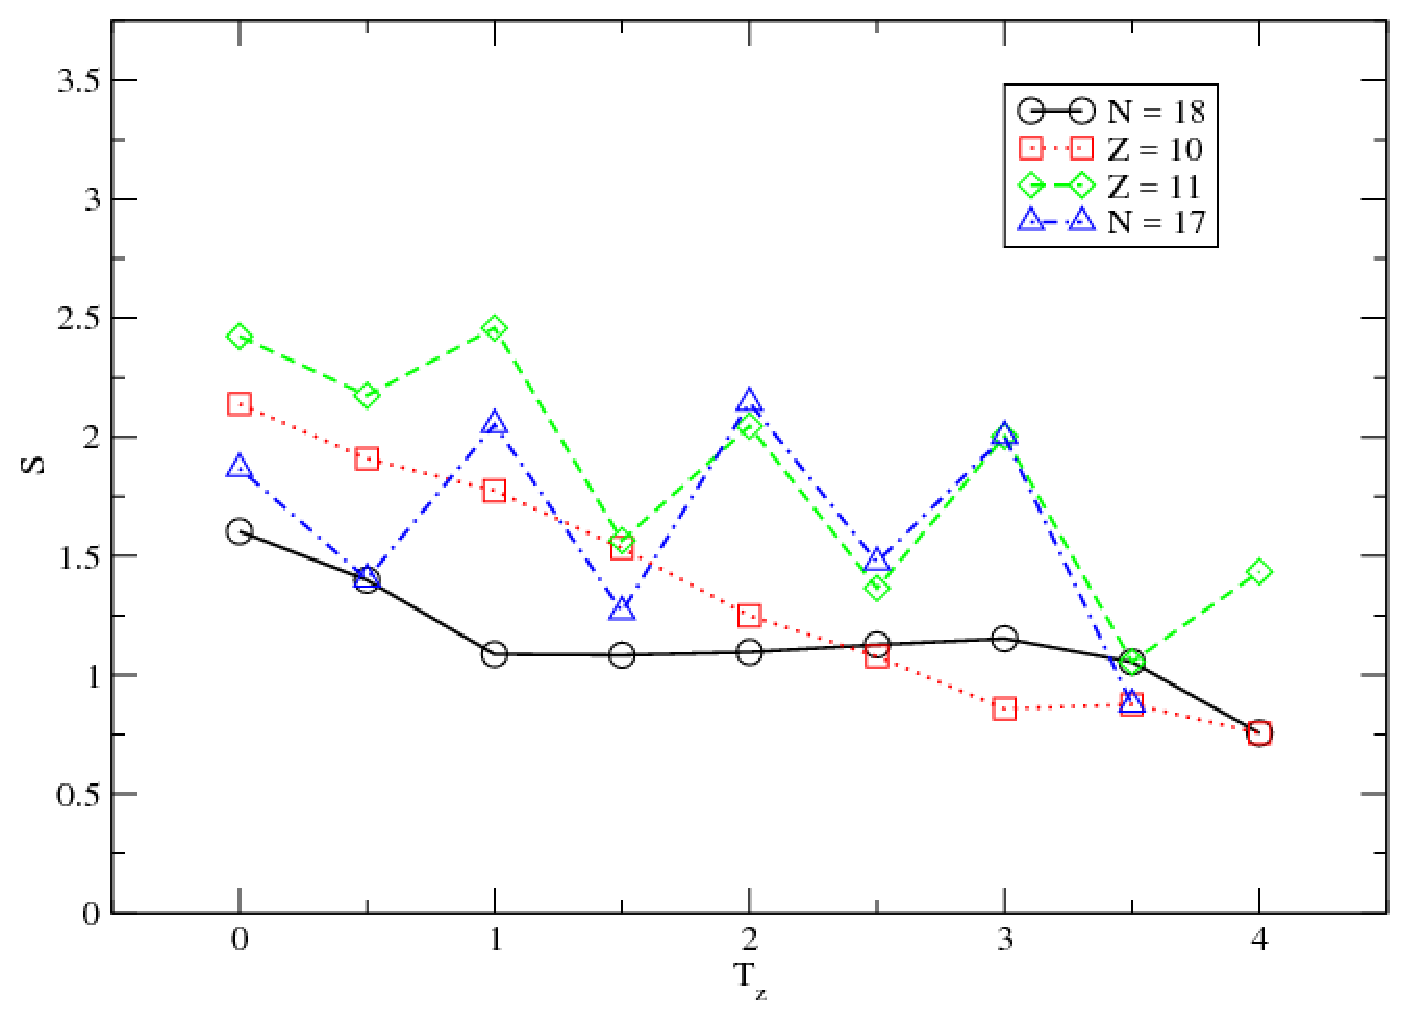
\includegraphics[width=.75\textwidth,clip]{Figures/s_vs_tz_sd}
        \caption{Entanglement entropy versus isospin for particle-hole conjugate nuclei in the
\textit{sd}-shell. Entanglement entropy tends to continuously decrease for even-even and even-odd 
numbers of protons and neutrons (see even-Z isotopes and even-N isotones), but 
to jump up for odd-odd nuclei (see odd-Z isotopes
and odd-N isotones).}
    \label{fig: tz1}
\end{figure}




\subsection{Dialing the Strength of the Proton-Neutron Interaction}

The shell-model code BIGSTICK to allows for scaling of the proton-neutron 
interaction term when working in the explicit proton-neutron 
formalism. Thus the two-body part of Hamiltonian is of the form
\begin{equation}
    H = H_{pp} + H_{nn} + \lambda H_{pn}.
\end{equation}
In BIGSTICK, this means scaling the two-body interaction
matrix elements by $\lambda$:
\begin{equation}
    \lambda\bra{ab}V^{(pn)}\ket{cd}
\end{equation}
We examined the relationship between the strength of the 
proton-neutron interaction and the relative proton-neutron 
entanglement entropy for the ground state of a number of 
nuclei. (See Figure \ref{fig: l28ne}.)
The scaling factor $\lambda$ was varied from zero, i.e.
no proton-neutron interaction at all, to an order of magnitude
above unity. A scaling factor of $\lambda=1$ is a fully realistic 
calculation.
The entanglement 
entropy will be zero when $\lambda$ is zero because in this
case there is no interaction between protons and neutrons. 
Essentially we have two separate and non-interacting 
model spaces. The entanglement entropy will increase as
the strength of the interaction increases. 

If our hypothesis that $N>Z$ nuclei converge faster in the 
proton-neutron formalism than $N=Z$ nuclei is correct, then 
we might expect different behavior in the
$S$ vs $\lambda$ curves for $N>Z$ and $N=Z$ nuclei.
In fact what we find is that the $S$ vs $\lambda$
curve for $N>Z$ nuclei falls below the one for $N=Z$ 
nuclei for nuclei of the same model space dimension.
Having the same model space dimension means that
the two nuclei will also have the same maximum 
proton-neutron entanglement entropy.
This is accomplished by comparing nuclei which are
particle-hole conjugates.

\begin{figure}[t]
    \centering
    \includegraphics[width=.75\textwidth,clip]{Figures/s_vs_lambda_28ne}
    \caption{Proton-neutron entanglement entropy as a function of the proton-neutron
two-body interaction matrix element scaling factor \boldmath$\lambda$. Entanglement entropy
is necessarily zero when $\lambda=0$. $\lambda<0$ value are non-physical but
shed light on the behavior of the coupling. $^{28}$Ne, with an unequal number 
of protons and neutrons, has the lowest entanglement entropy for values of 
$\lambda>0$ up until about seven times the realistic value of $\lambda=1$.}
    \label{fig: l28ne}
\end{figure}

Figure \ref{fig: l28ne} shows the dramatic difference between the 
$S$ versus $\lambda$ curves of nuclei with $N=Z$ versus $N>Z$.
$N>Z$ have significantly lower proton-neutron entanglement entropy
for values of $\lambda$ greater than zero up to about five to
seven times the realistic scaling of the proton-neutron
interaction. 


\section{Modified Nuclear Interactions}
We have shown that proton-neutron entanglement entropy is inversely correlated with
isospin; however it is not obvious why this is the case. 
In this section I summarize some of the attempts made to 
isolate the physics responsible for the behavior demonstrated 
in the previous chapter. To this end,
I recomputed the entanglement entropy versus proton-neutron interaction
strength (via the scaling factor $\lambda$) for several different
nucleon-nucleon interactions.

The first series of calculations were made with \textit{zero single particle energies}.
In this interaction we start with the fully realistic nuclear
interaction and then set the single particle energies equal 
to zero. In the many-body Hamiltonian,
\begin{equation}
    H = \sum_{ij} \epsilon_{ij}a^\dagger_ia_i + \sum_{ijkl} a^\dagger_ia^\dagger_jV_{ijkl}a_ka_l
\end{equation}
the single particle energies are $\epsilon_{ij}$.

The second series of calculations were made with \textit{traceless interactions} (see Figure \ref{fignmp}).
In this interaction we again start with the fully realistic nuclear
interaction and then remove the monopole terms in the two-body 
interaction. These are terms of the form\cite{Caurier}
\begin{equation}
    V_{mono} = \sum_{ab} \hat{n}_a(\hat{n}_b-\delta_{ab})U(ab),
\end{equation}
where $\hat{n}$ are number operators. These are related to shell structure.

The third series of calculations were made with only an attractive
quadrupole-quadrupole interaction\cite{Schuck} (see Figure \ref{figqq}). This interaction is derived from
the nuclear quadrupole moment\cite{Wong,Schuck},
\begin{equation}
    Q_{ij}=\int \rho(\vec{r})(3x_ix_j-r^2\delta_{id})d\vec{r},
\end{equation}
a tensor operator for which for microscopic expectation value for a system
of nuclear matter is given by\cite{Heyde,Schuck}
\begin{equation}
    Q_\alpha(J,M) = \bra{\psi_{JM}(r_i)}\sum_i(3x^\alpha_i-r_i^2)\ket{\psi_{JM}(r_i)},
\end{equation}
where $\alpha$ is the directional orientation of the quadrupole moment of 
interest.

The fourth series of calculations were made with an attractive pairing interaction (see Figure \ref{figpair}).
A problem arose when computing entanglement entropies for this interaction.
The pairing interaction is known to be highly degenerate, and in cases where the eigenstates are
nearly degenerate, the Lanczos method performs poorly. 
This is because the Lanczos method is susceptible to loss
of orthogonality of eigenstates due to numerical noise.
In order to counteract this, the two-body interaction
matrix elements were slightly modified. A very small random
interaction was added to the matrix elements in order to
desensitize the Lanczos algorithm to the degeneracies.
\begin{figure}[h]
    \centering

        \includegraphics[width=.75\textwidth,clip]{Figures/s_vs_lambda_nmp_ne}
        \caption{Entanglement entropy with a traceless interaction.}
        \label{fignmp}
\end{figure}
\begin{figure}
        \centering
        \includegraphics[width=.75\textwidth,clip]{Figures/s_vs_lambda_qq_ne}
        \caption{Entanglement entropy with an attractive quadrupole-quadrupole interaction.}
        \label{figqq}
\end{figure}

\begin{figure}
    \centering
    \includegraphics[width=.75\textwidth,clip]{Figures/s_vs_lambda_pair_ne}
    \caption{Attractive pairing interaction: Ne and PH-Conjugates.}
    \label{figpair}
\end{figure}

We also ran several trials with particle-hole conjugate nuclei 
with random two-body interactions (see Figure \ref{figrand1} and Figure \ref{figrand2}). This means that all of the
physics is removed and all that remains are properties of the 
model space. Because any given random interaction may not be particularly 
enlightening, we ran up to 1000 calculations with unique random
interactions and plotted a histogram of the ground state
entanglement entropy. In these calculations we lose the 
correlation between isospin and proton-neutron entanglement 
entropy. We often see normal distributions of the entanglement
entropy for a given nucleus, and two unique modes for the 
distributions within a particle-hole conjugate triplet.

\begin{figure}
    \centering
    \includegraphics[width=.75\textwidth,clip]{Figures/rand_s_ne}
    \caption{Random interactions exhibiting a bimodal distribution of entanglement entropy. No apparent
correlation between entanglement entropy and ratio of protons to neutrons.}
    \label{figrand1}
\end{figure}

\begin{figure}
    \centering
    \includegraphics[width=.75\textwidth,clip]{Figures/rand_s_ne_nmp}
    \caption{Random traceless interactions exhibiting a unimodal distribution of entanglement entropy. No
apparent correlation between entanglement entropy and ration of protons to neutrons. $N=Z$ nuclei have the
same entanglement entropy for all interactions, as expected.}
    \label{figrand2}
\end{figure}

This study failed to reveal the source of the isospin dependence of the
proton-neutron entanglement entropy. The phenomenon is not unique to
any of: the pairing interaction, the quadrapole-quadrapole interaction,
the full interaction with or without the monopole terms.

\section{Toy Model}

I constructed a toy model to investigate the behavior of 
entanglement entropy of coupled systems, in an attempt 
to better understand the behavior seen in real nuclei such as in Figure 
\ref{fig: l28ne}. In the toy model, I consider a subspace A and a subspace B, 
which together form a 
bipartite system $\mathcal{H}_{AB}=\mathcal{H}_A\otimes\mathcal{H}_B$.
$\mathcal{H}_{AB}$ is spanned by a coupled basis:
\begin{equation}
    \ket{i} = \ket{a}\ket{b} = \ket{a}\otimes \ket{b},
\end{equation}
where $\ket{a}$ are the basis states of $\mathcal{H}_A$ and 
$\ket{b}$ are the basis states of $\mathcal{H}_B$. A Hamiltonian operator of this
bipartite space could be written as
\begin{equation}
    \hat{H} = \hat{H}_A + \hat{H}_B + \hat{H}_{AB} 
\end{equation}
where $\hat{H}_A =\hat{h}_a \otimes \hat{1}$ is an operator which acts purely in the A space,
$\hat{H}_B=\hat{1}\otimes\hat{h}_b$ is an operator which acts purely in the B space and
$\hat{H}_{AB}=\hat{V}\otimes\hat{W}$ is an operator which acts on both spaces. 
We are interested in the behavior of the system as a function of the strength of the
coupling term $\hat{H}_{AB}$. I assume for convenience that we have already diagonalized $\hat{H}_A$
and $\hat{H}_B$. I choose single particle spaces with constant energy
spacing:
\begin{equation}
	E_a \equiv \hat{h}_A \ket{a} = a \epsilon 
\end{equation}
for $a=1,..,N$ and $\epsilon = const.$, and similarly for $\hat{H}_B$.

For $\hat{H}_{AB}$ I choose an operator which is the tensor product of an 
operator $\hat{V}$ in $\mathcal{H}_A$ and an operator $\hat{W}$ in $\mathcal{H}_B$. I am only interested in
the behavior of the system as a function of the strength of the interaction between
the subsystems, so the exact structure of each subsystem is not important. Therefore, 
I simply choose to fill these two matrices with a random Gaussian number generator. I 
symmetrically fill an $N\times N$ matrix with random numbers centered at zero with a
standard deviation of $2\sigma$ for the diagonal matrix elements, 
and $\sigma$ for the off-diagonal matrix, a standard practice for generating 
real, symmetric random matrices. Finally, I include a two-body matrix elements 
(TBME) scaling factor $\lambda$:
\begin{equation}
	\hat{H}_{AB} = \lambda\hat{V}\otimes \hat{W}
\end{equation}
It is now straightforward to calculate the matrix elements of the Hamiltonian.
As above, let $a$, $a'$ label the proton states and $b$, $b'$ 
label the neutron states. These run from 1 to $N$. Now let $i = a + N(b-1)$ label 
the many-body state, which runs from 1 to $N^2$. Then
\begin{equation}\label{eq:1}
	\bra{i'}\hat{H}\ket{i} =     
	H_{i',i} = \delta_{a'a}\delta_{b'b}(E_a+E_b)+\lambda V_{a'a} W_{b'b}.
\end{equation}
$V_{a'a}$ and $W_{b'b}$ are real, symmetric, $N \times N$ 
random matrices with Gaussian distributions:
\begin{equation}
    P(V_{aa'}) \sim exp\Big(-\frac{V_{aa'}^2}{2\sigma^2(1+\delta_{a'a})}\Big),
\end{equation}
a Gaussian distribution of $\sigma$ for the off-diagonals and $2\sigma$ for the diagonals.

Once we diagonalize the model Hamiltonian, we want to quantify
how the entanglement entropy is affected by the coupling-
term scaling factor $\lambda$ and by the two interactions
are the same $W=V$ or different $W\neq V$. This is meant to
model the behavior of the nuclear Hamiltonian when and its
distinct $S_{pn}$ versus $\lambda$ curves for when
the number of protons is the same or different from 
the number of neutrons. 

Suppose that we diagonalize the Hamiltonian and that
\begin{equation}
\hat{H} \ket{\psi}_i = E_i \ket{\psi}_i
\end{equation}
defines our $N^2$ eigenstates. Any given state can be written as 
\begin{equation}
\ket{\psi} = \sum_i c_i \ket{i} = \sum_{a,b} c_{ab} \ket{a}\ket{b},
\end{equation}
and so the reduced density matrix $\rho_A$  of $\ket{\Psi}$ is the partial trace, 
\begin{equation}
    \rho_A = tr_a\ \rho.
\end{equation}
Given our choice of indexing, this is computed as
\begin{equation}
    \rho_p(a',a) = \sum_{b=1}^N c_{a'b}c_{ab}^*.
\end{equation}
We can now define the proton-neutron entanglement 
entropy of the state described by $\rho$ to be the 
\textit{von Neumann} entropy of the reduced density 
matrix $\rho_p$,
\begin{equation}
    S_{pn} = -tr \rho_p\ \ln \rho_p.
\end{equation}
If we first diagonalize $\rho_p$ to find its $N$ eigenvalues 
$\gamma_i^2$ then the entanglement entropy becomes
\begin{equation}
    S_{pn} = - \sum_{i=1}^N \gamma_i^2\ \ln \gamma_i^2.
\end{equation}
This quantity measures the entanglement entropy, or 
the mixing of quantum bits, of the two subspaces in a 
given state of the Hamiltonian.

In the first adaption of this toy model we has Hamiltonian matrix elements
exactly as they appear in equation (\ref{eq:1}).
Here, $\epsilon=1$, $\sigma=1$, and 
two curves are plotted: one in which the random matrices 
$V$ and $W$ are the same and one in which they are different. 
In these models we saw that when the two interactions $W$ and $V$ are the same, the 
entanglement entropy tends towards some finite non-zero value, 
whereas when $W$ and $V$ are different, the 
entanglement entropy falls off to zero. This tells us that the entanglement 
entropy can differ between two systems of the same dimension depending on 
the similarity of the interactions acting between the subspaces. Mathematically this has to do with the 
orthogonality of the eigenstates of the interactions within each subspace.
In another adaption of the model, we start 
with two identical subspaces and then slowly change 
one of the subspaces to be different from the original. 
\begin{equation}\label{modeld}
	H = E^V + E^W + \lambda(V\otimes(V+\delta W))
\end{equation}
In doing so we can see in Figure \ref{opt3} that as the two interactions diverge, 
the entanglement entropy of the system falls off from its
maximum convergent value. 
When the perturbative parameter $\delta=0$, equation (\ref{modeld})
reduces to equation (\ref{eq:1}) for the case when $W=V$.

\begin{figure}
    \centering
    \includegraphics[width=	.75\textwidth,clip]{Figures/toymodel1delta}
    \caption{Toy Model with perturbative variance of the interaction $W$ away from $V$. 
    The subspaces containing the $V$ interaction has the same dimensions as the 
    subspace containing the $W$ interaction. See equation (\ref{modeld}).}
    \label{opt3}
\end{figure}

In an attempt to get convergence to non-zero entanglement entropies
when $W\neq V$, which is what we see in the nuclear calculations, I suggested 
the following Hamiltonian on the grounds that a constant term may 
prevent the entanglement entropy from converging to zero when the 
two species of interactions are different:
\begin{equation}
    H_{i',i} = \delta_{a'a}\delta_{b'b}(E_a+E_b)+\lambda
\big( V_{a'a} W_{b'b} + V_{a'a} + W_{b'b} \big ),
\end{equation}
which implicitly is a Hamiltonian of the form
\begin{equation}
    H = E^V + E^W + \lambda ( V\otimes W + V\otimes I + I \otimes W ),
\end{equation}
where $E$ is diagonal. By using an explicitly non-separable interaction,
we obtained the desirable feature than $W\neq V$ curves converged to
non-zero entanglement entropy. However, curves generated with different
random number generator seeds produced varying results, some exhibiting
anomalous spikes in entropy near the origin. 

The next most obvious 
adaption was to simply include a several terms in the coupling part of the Hamiltonian:
\begin{equation}
    H_{i',i} = \delta_{a'a}\delta_{b'b}(E_a+E_b)+\lambda\big( 
\sum_i V_{a'a}^i W_{b'b}^i  \big ),
\end{equation}
which is a Hamiltonian of the form:
\begin{equation}
    H = E^{(V)} + E^{(W)} + \lambda (\sum_i V_i \otimes W_i ),
\end{equation}
where each 
The results of this toy model are shown in Figure \ref{best}.
This version of the toy model has the following 
features: 
\begin{itemize}[noitemsep]
\item Entanglement entropy goes to zero at the origin
\item Dependence on the random number generator seed goes down
    with the number of terms in the sum
\item Entanglement entropy convergences to nonzero entanglement 
    entropies at large $\lambda$ for different 
subspaces, and 
\item Very few anomalous features, such as spikes in entanglement entropy
\end{itemize}

However, the model still doesn't have the same features as the
realistic proton-neutron entanglement entropy, namely, symmetric
entanglement entropy curves when the both species' interactions
are identical, and, when the interactions are different: lower entanglement entropy 
for positive $\lambda$ and higher entanglement entropy for negative $\lambda$.
See Figure \ref{best} (a) and (b) for comparison.
Several dozen other toy model Hamiltonians were investigated, including those with different 
single species interactions, and models with different dimensions. However, I
 failed to find a model which reliably produces $S$ versus $\lambda$ curves with 
the same topology as in the nuclear Hamiltonian.
\begin{figure}[t]
    \centering
	\subfigure[]{
		\includegraphics[width=.75\textwidth,clip]{Figures/toymodel3}
	}
	\qquad
	\subfigure[]{
		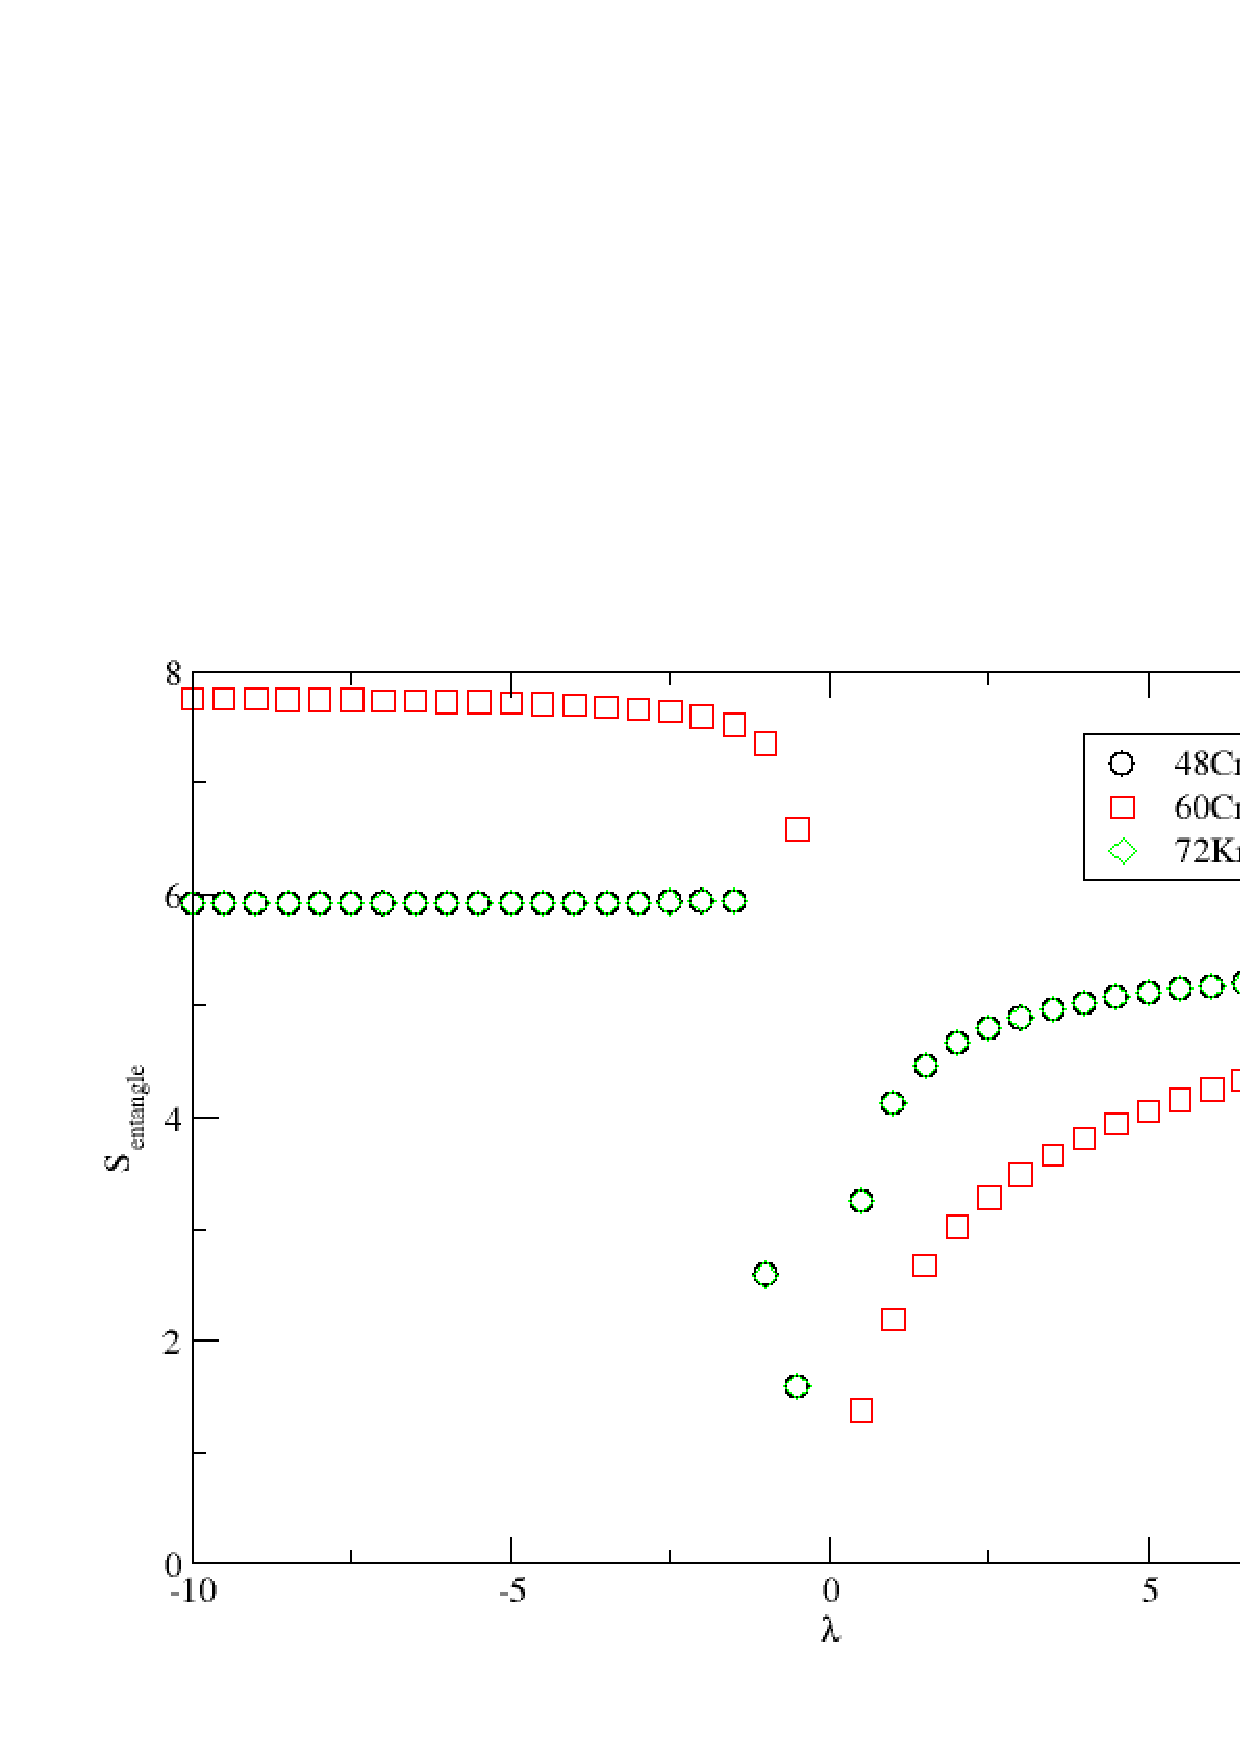
\includegraphics[width=	.85\textwidth,clip]{Figures/s_vs_lambda_48crnmp}
	}
	\caption{Entanglement entropy $S$ versus scaling factor $\lambda$ for (a) toy model 
    with non-separable two-body terms, and (b) nuclei in the \textit{pf}-shell with a traceless interaction.}   
	\label{best}
\end{figure}


\section{Summary on Entanglement Entropy}
We investigated the properties of the proton-neutron entanglement entropy,
which is an indicator used to determine whether or not certain wavefunctions
could be represented more efficiently in some basis. We showed that nuclei with
unequal numbers of protons and neutrons have a lower entanglement entropy, which
means that $N>Z$ nuclei may have even more efficient representations. We
attempted to understand the properties of the entanglement entropy, but more 
investigation is needed. The toy model we investigated tells us that the phenomenon
of higher entanglement entropy in systems with identical subspaces is more
ubiquitous than the nuclear many-body problem. Moving on from this section,
readers should keep in mind that we have evidence for the existence of 
efficient representations of our nuclear wavefunctions, but have yet to 
inquire about which basis will yield these efficient representations. This will
be addressed in the next chapter.






